\documentclass[11pt]{article}
\usepackage[letterpaper,margin=1in]{geometry}
\usepackage[T1]{fontenc}
\usepackage{mathptmx}
\usepackage{amsmath,amssymb}
\usepackage{graphicx}
\usepackage{booktabs}
\usepackage[font=small,labelfont=bf]{caption}
\usepackage[numbers,sort&compress]{natbib}
\usepackage{xcolor}
\usepackage{microtype}
\usepackage{authblk}
\usepackage[colorlinks=true,linkcolor=blue!50!black,citecolor=blue!50!black,urlcolor=blue!50!black]{hyperref}
\setlength{\emergencystretch}{3em}
\renewcommand{\baselinestretch}{1.12}
\newcommand{\LIO}{\texorpdfstring{LaInO$_3$}{LaInO3}}
\newcommand{\BSO}{\texorpdfstring{BaSnO$_3$}{BaSnO3}}
\newcommand{\ntot}{n_\mathrm{tot}}
\newcommand{\xmax}{x_\mathrm{max}}
\makeatletter\newcommand{\inputrows}[1]{\@@input #1 }\makeatother

\title{Immobile electrons at frozen gate charge: what the transport data of electrolyte-gated \LIO/\BSO\ allow}
\author{Gracen Ownby}
\affil{University of Oklahoma, Norman, Oklahoma, USA}
\date{\small 14 October 2026}

\begin{document}
\maketitle

\begin{abstract}
In the electrolyte-gated \LIO/\BSO\ two-dimensional electron gas of Lee \emph{et al.}, each gate voltage is set above the freezing point of the ionic liquid and the sample is then cooled, so the total charge and the ionic and defect configuration are fixed below it. Yet between 150 and 2~K the Hall density falls by 10, 15, 26 and 40\% at 4, 5, 7 and 8~V. We ask what the published Hall, resistance and magnetoresistance data allow, using a self-consistent subband model and a multisubband transport calculation. Coupled subbands in a magnetic field are exactly equivalent to independent Drude channels, so we search all two- and three-channel sets that reproduce the measured conductance and Hall density at 2~K. At 7~V, a magnetoresistance flat to 0.1\% between 2 and 7~T then requires about a quarter of the electrons (at least 22\% in three channels; 26--29\% in two, with mobilities below 50~cm$^2$/Vs) to sit in states with mobility below 200~cm$^2$/Vs, against about 1200~cm$^2$/Vs for the rest. At 5~V the data cannot decide. Coulomb scattering by the gate-induced positive charge next to the interface, which electrostatics requires, makes the subbands differ in mobility by less than a factor of two and lowers the Hall density by at most 4\% at 7--8~V, with a magnetoresistance consistent with the data. So the identified scattering produces no such slow channel: at 7~V about $2\times10^{13}$~cm$^{-2}$ electrons are effectively immobile, most likely trapped or localized. Below 50~K the conductance falls with the Hall density by 9--24\% at 5--8~V, while the field-suppressible weak-localization correction is only 2--4\%. A trap release on warming with emission barriers of 6--150~meV would need about $10^{14}$~eV$^{-1}$cm$^{-2}$ of trap states, plausible for $10^{14}$~cm$^{-2}$ charged centres at the interface. The conductance also bounds how close random point charges can be to the interface; at 8~V the bound and the electrostatic limit agree within a factor of about 1.5 for clean \BSO\ and singly charged centres.
\end{abstract}

\section{Introduction}
The two-dimensional electron gas (2DEG) at the polar interface between \LIO\ and \BSO\ combines a polarization-induced density of a few $10^{13}$~cm$^{-2}$ with the high mobility of \BSO\ \cite{Kim2016LIO,Kim2019LIO,Aggoune2021}. Lee \emph{et al.} gated it with the ionic liquid DEME-TFSI on a 5~nm \LIO\ cap, grown by pulsed laser deposition on 110~nm of \BSO\ grown by molecular-beam epitaxy on MgO \cite{Lee2024LIO}. Each gate voltage $V_{GS}$ was applied at 220~K, where the liquid is mobile; the sample was then cooled to 2~K at constant bias and measured while warming. The liquid has its glass transition near 182~K \cite{McCann2015}. Below it the ions do not move, and neither does the positive charge that balances the gated electrons. A companion study \cite{OwnbyMAT02} found that this positive charge must sit within about one \LIO\ unit cell of the interface to keep electrons out of the cap. It cannot be the layer of liquid ions on the cap surface, 5~nm away; it must be charged defects formed electrochemically during gating, such as oxygen vacancies, whose number is set at 220~K. Lee \emph{et al.} also report an irreversible change of the sheet resistance after gating, consistent with such electrochemistry.

Their Fig.~3 gives the sheet resistance from 2 to 220~K and the Hall density $n_H$ and mobility $\mu_H$ at 2, 10, 50, 100 and 150~K for $V_{GS}=0$--8~V; their Fig.~5a gives the magnetoresistance at 2~K up to 7~T for 0, 1, 3, 5 and 7~V. At 8~V the Hall density reaches $1.08\times10^{14}$~cm$^{-2}$ at 150~K and the Hall mobility 2000~cm$^2$/Vs at 2~K. Lee \emph{et al.} note that the Hall density falls on cooling at high bias, a point they leave open, and attribute a slow rise of the resistance at low temperature to weak localization.

With the total charge fixed, electrons cannot disappear. Either the Hall measurement undercounts them, or some of them stop contributing to the current. For parallel channels, $n_H=(\sum_in_i\mu_i)^2/\sum_in_i\mu_i^2$ equals the electron density only when all channels have the same mobility \cite{Ziman1972}, and at $10^{14}$~cm$^{-2}$ the interface has two or three occupied subbands. The mobility differences that lower $n_H$, however, also produce a positive classical magnetoresistance. Here we use this link, with a self-consistent subband model and a multisubband transport calculation, to find what kind of electron distribution the data require. We also use the measured conductance to bound where the gate-induced charge can sit.

\section{Data}\label{sec:data}
We digitized three figures of Ref.~\cite{Lee2024LIO}: Fig.~3b (Hall density and mobility); Fig.~3a (sheet resistance) for 5--8~V, where the curves are separated; and Fig.~5a (magnetoresistance at 2~K) for 3, 5 and 7~V. The digitization is accurate to a few per cent on the logarithmic axes and to about 0.1 percentage point on the magnetoresistance. At 2~K and 8~V we read $6.49\times10^{13}$~cm$^{-2}$ and 1985~cm$^2$/Vs, against $6.52\times10^{13}$~cm$^{-2}$ and 1999~cm$^2$/Vs quoted in the text of Ref.~\cite{Lee2024LIO}. The 6~V Hall markers at 2 and 10~K are hidden behind the 7~V markers, and a second reading of the 6~V series gives different values, so we do not use the 6~V Hall data.

For parallel Drude channels the conductance is $\sigma=e\,n_H\mu_H$ exactly. The resistance of Fig.~3a is 1.12--1.48 times $1/(e\,n_H\mu_H)$, a factor that grows with gate voltage and changes with temperature. Both were measured on the same Hall bar, so the difference is not geometric, and we cannot explain it. Their relative temperature dependence agrees: between 50 and 2~K the resistance rises by 9.7, 18.5 and 26.8\% at 5, 7 and 8~V in Fig.~3a and by 9.8, 23.9 and 32.0\% in the Hall data (Fig.~\ref{fig:data}b), so the conductance falls by 9--24\%. The rise is not monotonic in gate voltage. At 6~V the resistance of Fig.~3a falls by 10\% between 50 and 2~K, and at 4~V the Hall data give a fall of 42\% with a Hall mobility rising by 86\%.

Since $n_H\le\ntot$, the largest measured Hall density, at 150~K, is a lower bound on the electron density $\ntot$; we use $\ntot=n_H(150\ \mathrm{K})$. At 2~K the Hall density is 90, 85, 74 and 60\% of it at 4, 5, 7 and 8~V (Fig.~\ref{fig:data}a), a shortfall of 0.4, 0.7, 1.9 and $4.3\times10^{13}$~cm$^{-2}$. At 2--3~V the sheet resistance is 2.5--3~k$\Omega$ ($k_Fl\approx10$), close to the metal--insulator crossover, so we concentrate on 4--8~V.

\begin{figure}[t]
\centering
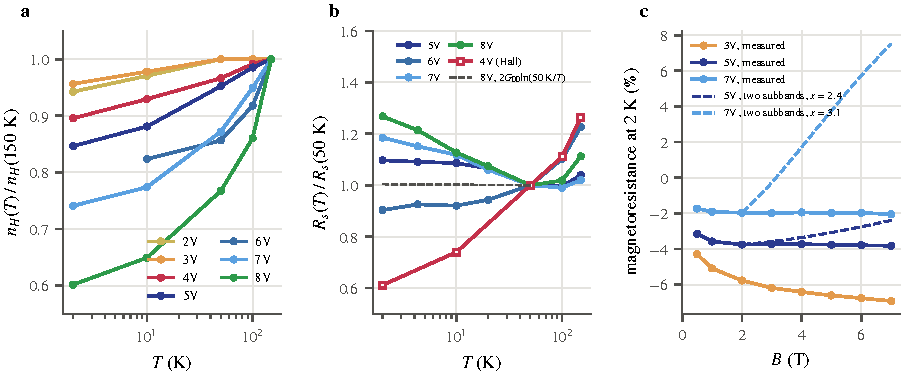
\includegraphics[width=\textwidth]{figures/fig1_data.pdf}
\caption{Data of Lee \emph{et al.} \cite{Lee2024LIO}, digitized. (a) Hall density relative to its 150~K value, with the total charge frozen. (b) Sheet resistance relative to 50~K, from their Fig.~3a (5--8~V) and from $1/(e\,n_H\mu_H)$ (4~V). Dashed: the 8~V curve if the conductance fell by $2G_{00}\ln(50\,\mathrm{K}/T)$, a typical size for weak localization and the interaction correction together. (c) Magnetoresistance at 2~K (their Fig.~5a), mean of $\pm B$. Dashed: the classical magnetoresistance, added to the measured value at 2~T, of two independent subband channels with the model's populations, the measured conductance and the mobility ratio $x$ that reproduces the 2~K Hall density at low field with the upper subbands more mobile.}
\label{fig:data}
\end{figure}

\section{Model}\label{sec:model}
\emph{Subbands.} The interface is described by the self-consistent Schr\"odinger--Poisson model of Refs.~\cite{OwnbyMAT01,OwnbyMAT02}, implemented in qwkit \cite{qwkit}. Its ingredients are:
\begin{itemize}
\item a Kane-nonparabolic conduction band of \BSO\ (mass $0.19\,m_0$, nonparabolicity 0.56~eV$^{-1}$, static permittivity 20);
\item a 5~nm \LIO\ cap (offset 1.6~eV, mass $0.46\,m_0$);
\item deep acceptors in the \BSO, depleting over a width set by Fermi-level pinning;
\item a fixed interface charge that gives $5\times10^{12}$~cm$^{-2}$ without gating.
\end{itemize}
We consider strongly compensated \BSO\ ($N_A=5\times10^{19}$~cm$^{-3}$, as reported for films grown by pulsed laser deposition \cite{Kim2019LIO}) and clean \BSO\ ($10^{18}$~cm$^{-3}$). The added positive charge sits next to the interface, as Ref.~\cite{OwnbyMAT02} requires; by Gauss's law the \BSO\ side does not depend on its exact place while the cap is empty. Ten subbands enter at 2~K on a 0.5~\AA\ grid. In compensated \BSO\ the second subband is occupied only above $6.5\times10^{13}$~cm$^{-2}$ and holds 3 and 12\% of the electrons at 7 and 8~V. In clean \BSO\ the ground subband holds 84, 81, 79 and 76\% at 4, 5, 7 and 8~V. Its mean distance from the interface is 0.7--1.1~nm, against 2.0--3.0~nm for the second subband.

\emph{Scattering.} At 2~K we compute the momentum relaxation times of all occupied subbands at the Fermi level from the coupled Boltzmann equations of Siggia and Kwok \cite{SiggiaKwok1970},
\begin{equation}
1=\sum_j\left[\frac{\tau_i}{\tau^{(0)}_{ij}}-\frac{v_j}{v_i}\,\frac{\tau_j}{\tau^{(1)}_{ij}}\right],
\end{equation}
with Fermi velocities $v_i=\hslash k_i/m_i$ and nonparabolic density-of-states masses $m_i$. The matrix elements are those of point charges in the Born approximation, screened in the static random-phase approximation with the intrasubband polarizabilities of all occupied subbands \cite{SiggiaKwok1970,AFS1982}. The scatterers are:
\begin{enumerate}
\item all of the positive charge added by gating, $\ntot+N_\mathrm{dep}-\sigma_P$, as random point charges $Ze$ ($Z=1$, 2) in a plane a distance $d=1$--32~\AA\ inside the cap. They act through the cap--\BSO\ boundary, with cap permittivity $\varepsilon_\mathrm{cap}=24$, 38 or 50: the bare potential in the \BSO\ is reduced by $2\varepsilon/(\varepsilon+\varepsilon_\mathrm{cap})$, and the 2DEG's own screening acquires an image term;
\item the ionized acceptors of the depletion layer;
\item charged threading dislocations at $10^{10}$--$10^{11}$~cm$^{-2}$, typical of \BSO\ grown by molecular-beam epitaxy \cite{Paik2017}, whose bare potential acts only within a subband \cite{Jena2000};
\item interface roughness in the finite-barrier form \cite{AFS1982}, as an order-of-magnitude check.
\end{enumerate}
The relaxation times agree with an independent quadrature of the single-subband integral to $10^{-3}$, and with a direct angular solution of the coupled Boltzmann equations to $10^{-9}$. The mobilities change by less than 0.2\% between 32 and 128 angles and on a 0.25~\AA\ grid, and by 0.7--1.5\% between 10 and 14 subbands.

\emph{Magnetotransport.} For isotropic subbands the drift velocity $u_i$ of each subband obeys
\begin{equation}
m_i\sum_jG_{ij}u_j=-e(E+u_i\times B),
\end{equation}
with $G$ the relaxation matrix of the coupled Boltzmann equations. Detailed balance makes $G$ similar to a symmetric matrix, so the subbands can be replaced exactly by independent Drude channels, the eigenmodes of $m_iG_{ij}$, with non-negative weights that sum to $\ntot$; we verified this numerically to $10^{-9}$. Intersubband scattering therefore changes the weights and mobilities of the channels, which can suppress or enhance the magnetoresistance relative to the subbands taken as independent \cite{Zaremba1992}, but it cannot produce a Hall response outside what some set of independent channels gives. Lee \emph{et al.} obtained $n_H$ from Hall resistances that were linear up to 7~T; we fit a straight line through the origin over 0.25--7~T to model the same procedure.

\section{Results}
\subsection{What the magnetoresistance requires}\label{sec:mr}
At 2~K the magnetoresistance at 5 and 7~V (Fig.~\ref{fig:data}c) has a weak-localization cusp below 1~T and is then flat: between 2 and 7~T it changes by $-0.07$ and $-0.08$ percentage points. If the upper subbands were the more mobile ones, the 2~K Hall density would need a mobility ratio $x=2.4$ (5~V) or 3.1 (7~V). Two independent subband channels with the model's populations and the measured conductance would then raise the magnetoresistance between 2 and 7~T by 1.3 and 9.5 points (dashed in Fig.~\ref{fig:data}c).

The general question is which channel sets reproduce the measured conductance and fitted Hall density while keeping the rise between 2 and 7~T within the measured change plus a tolerance. We take tolerances of 0.5 and 1.0 point. They cover the digitization, a remaining weak-localization tail (about $-0.2$ and $-0.05$ points at 5 and 7~V, scaled from the 3~V curve by the conductance), and the parabolic negative magnetoresistance of the electron--electron interaction (a few tenths of a point at 7~V). We sampled two- and three-channel sets with random weights and mobilities between 1 and 30\,000~cm$^2$/Vs, constrained to the measured values (Table~\ref{tab:sum}, Fig.~\ref{fig:bounds}b).
\begin{itemize}
\item \emph{7~V.} Every acceptable set has a slow channel. With two channels, 26--29\% of the electrons must have a mobility below 22~cm$^2$/Vs (tolerance 0.5) or 48~cm$^2$/Vs (tolerance 1.0). With three channels, at least 22--24\% must be slower than 200~cm$^2$/Vs. The other electrons then carry the current with about 1200~cm$^2$/Vs. Sets with a fast minority channel either bend the magnetoresistance or, when that channel saturates below 2~T, bring the fitted Hall density up to $\ntot$.
\item \emph{5~V.} The magnetoresistance does not constrain the sets ($\mu B\approx0.3$ at 7~T): acceptable sets include fast-minority, slow-minority and slow-majority channels, with no slow channel required.
\end{itemize}
A slow channel holding a quarter of the electrons at 7~V could be a subband 25--50 times less mobile than the others, or electrons in localized states; the transport data alone cannot tell which. Paramagnetic or Kondo-like negative magnetoresistance from spin-carrying centres could in principle cancel a positive classical rise. Doing so at both 5 and 7~V over 2--7~T would need fine tuning.

The magnetoresistance also measures weak localization. The negative cusp saturates at $-3.8$\% (5~V) and $-2.0$\% (7~V), so the whole field-suppressible correction to the 2~K conductance is 2--4\%. The resistance, by contrast, rises between 50 and 2~K by 10\% at 5~V and 19--24\% at 7~V. We write the conductance change as
\begin{equation}
\sigma(50\,\mathrm{K})-\sigma(2\,\mathrm{K})=A\,G_{00}\ln 25,\qquad G_{00}=\frac{e^2}{2\pi^2\hslash},
\end{equation}
and find $A=5$--7 at 5~V, 37--63 at 7~V and 98--166 at 8~V, with $k_Fl=56$--533. Weak localization and the electron--electron interaction correction together give $A$ of a few, at most about 4--6 with several subbands and strong dephasing \cite{AltshulerAronov1980,LeeRamakrishnan1985}. Their relative size also falls as $1/k_Fl$, whereas here it grows with $k_Fl$. The resistance rise at 7--8~V is therefore not a quantum correction; at 5~V the comparison is inconclusive. Weak localization leaves the Hall coefficient unchanged, and the interaction correction changes it by twice the relative conductance change \cite{AltshulerAronov1980,LeeRamakrishnan1985}, which would make the Hall mobility rise as the conductance falls. Between 50 and 2~K, the Hall mobility instead changes by $+3$, $-5$ and $-4$\% at 5, 7 and 8~V, while the Hall density falls by 11, 15 and 21\%.

\subsection{What the gate-induced charge does}\label{sec:coulomb}
Electrostatics places the positive charge that balances the gated electrons within a few \aa ngstr\"oms of the interface \cite{OwnbyMAT02}, and at these densities it dominates the elastic scattering that we can identify. With the charge 1--6~\AA\ inside the cap ($\varepsilon_\mathrm{cap}=24$), it makes the upper subbands more mobile than the ground subband, which overlaps it most, by a factor of:
\begin{itemize}
\item 1.46--1.72 at 4~V;
\item 1.67--1.86 at 5~V;
\item 1.32--1.57 at 7~V;
\item 1.42--1.76 at 8~V.
\end{itemize}
The ratio falls towards 1, and below, as the charge moves further away. The model mobilities are higher than the measured ones, so part of the scattering is unidentified: 70--95\% of it at 5~V, less at 7--8~V. We add it in two limits that bracket its effect: all rates scaled by one factor, which keeps the model's mobility ratios, or an extra rate equal for all subbands, which pushes them towards 1. In both, the conductance is matched to the measured 2~K value; we keep only distances at which the model conductance is not already below it. With the coupled magnetotransport, the Coulomb scattering then lowers the Hall density to 0.92--1.00 (5~V), 0.97--0.99 (7~V) and 0.96--1.00 (8~V) of $\ntot$ (Fig.~\ref{fig:bounds}a), with a magnetoresistance rise of at most 0.3, 0.6 and 1.4 points between 2 and 7~T. That is a deficit of 0--8\% at 5~V, against 15\% observed, and at most 3--4\% at 7--8~V, against 26--40\%.

Charged dislocations scatter most strongly the subbands with the smallest Fermi wavevector and lower the ratio, to 0.32--1.25 at 4~V and 1.00--1.43 at 8~V for $10^{10}$--$10^{11}$~cm$^{-2}$. Interface roughness leaves it at 1.3--1.9. In compensated \BSO\ the barely occupied second subband scatters more strongly than the ground subband ($x=0.1$--0.9), but holds too few electrons (3--12\%) to form the slow channel that 7~V requires. None of the scatterers we can identify makes a quarter of the electrons 25--50 times slower than the rest.

\begin{table}[t]
\centering
\small
\caption{Clean \BSO, by gate voltage. Columns: electron density $\ntot=n_H(150\,\mathrm{K})$ ($10^{13}$~cm$^{-2}$); measured $n_H/\ntot$ at 2~K; ground-subband fraction $f_1$; smallest weight of channels slower than 200~cm$^2$/Vs among the three-channel sets that reproduce the 2~K conductance, Hall density and flat magnetoresistance (tolerance 0.5 / 1.0 point; magnetoresistance measured at 5 and 7~V only); $n_H/\ntot$ from Coulomb scattering by the gate-induced charge at the measured conductance (both limits, $Z=1$, 2, $\varepsilon_\mathrm{cap}=24$); smallest distance $d_\mathrm{min}$ (\AA) of that charge compatible with the measured conductance, from the Hall data / from Fig.~3a of Ref.~\cite{Lee2024LIO}, for $Z=1$ and $Z=2$; largest distance $\xmax$ (\AA) allowed by electrostatics at 150~K for $\varepsilon_\mathrm{cap}=24$ \cite{OwnbyMAT02}.}
\label{tab:sum}
\begin{tabular}{ccccccccc}
\toprule
$V_{GS}$ (V) & $\ntot$ & $n_H/\ntot$ & $f_1$ & slow weight & $n_H/\ntot$, Coulomb & $d_\mathrm{min}$, $Z=1$ & $d_\mathrm{min}$, $Z=2$ & $\xmax$ \\
\midrule
\inputrows{table1.tex}
\bottomrule
\end{tabular}
\end{table}

\subsection{Where the gate-induced charge can be}\label{sec:where}
The conductance limits how strongly the gate-induced charge can scatter. Suppose other scattering only adds to it and the subband populations do not change with temperature. Then the conductivity mobility limited by that charge alone, $\mu_\sigma=\sum_i(n_i/\ntot)\mu_i$, cannot be smaller than the largest measured $\sigma/(e\ntot)$ between 2 and 150~K. From the Hall data this bound is 503, 392, 1109 and 1578~cm$^2$/Vs at 4, 5, 7 and 8~V; from the resistance of Fig.~3a it is 304, 814 and 1069~cm$^2$/Vs at 5, 7 and 8~V. If a quarter of the electrons are immobile, the bound on the rest is higher still, so these values are conservative.

Figure~\ref{fig:bounds}c shows $\mu_\sigma$ against the distance of the charge at 8~V, with the permittivity entering the scattering and the electrostatic limit consistently:
\begin{itemize}
\item At 4--5~V the bound is met even at 1~\AA.
\item At 7~V it requires $d\ge2.8$ or 1.6~\AA\ for $Z=1$ (Hall or Fig.~3a conductance) and $d\ge5.5$ or 4.2~\AA\ for $Z=2$, well inside the electrostatic limit of 11.6~\AA.
\item At 8~V it requires $d\ge4.9$ or 3.5~\AA\ for $Z=1$ and 7.7 or 6.0~\AA\ for $Z=2$. Electrostatics allows 4.3~\AA\ for $\varepsilon_\mathrm{cap}=24$, and 6.3 and 7.9~\AA\ for 38 and 50.
\end{itemize}
For singly charged centres, the two limits meet within a factor of 1.2 in the scattering rate at the measured cap permittivity. Doubly charged centres would need their rate reduced 1.6--2.4 times, or a cap permittivity of at least 38. Spatial correlation of the charged centres reduces their scattering in this way, strongly so at high density \cite{Efros1990,Buks1994}. These numbers come from an envelope-function model at the edge of its validity for charges a few \aa ngstr\"oms from the interface, and the electrostatic limit treats the charge as a smeared sheet, so we read them as consistent within a factor of about 1.5.

For strongly compensated \BSO, in contrast, the conductance at 8~V requires $d\ge6.5$--12.3~\AA\ for $\varepsilon_\mathrm{cap}=24$, while electrostatics allows 1.8~\AA, so the scattering rate would have to be reduced 3--8 times. For $\varepsilon_\mathrm{cap}=50$, $d\ge3.6$--8.5~\AA\ against 2.8~\AA, a factor of 1.2--2.9. Roughness with correlation lengths of 3~nm or less would by itself bring the conductivity mobility below the 7--8~V bounds. At 6--20~nm it lowers $\mu_\sigma$ by 3--19\% for 2~\AA\ steps and by 9--48\% for 4~\AA\ steps.

\begin{figure}[t]
\centering
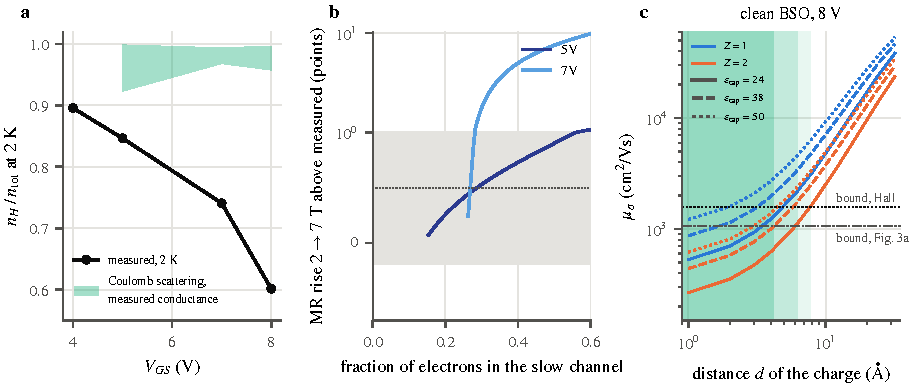
\includegraphics[width=\textwidth]{figures/fig2_bounds.pdf}
\caption{(a) Hall density relative to $\ntot$ at 2~K: measured, and the range produced by Coulomb scattering by the gate-induced charge at the measured conductance (both limits for the unidentified scattering; $Z=1$, 2; $\varepsilon_\mathrm{cap}=24$). (b) Two channels that reproduce the measured 2~K conductance and fitted Hall density, as a function of the fraction of electrons in the slower one: rise of the classical magnetoresistance between 2 and 7~T above the measured change. Shaded: within a 1.0-point tolerance; dotted: 0.5 point. At 7~V only a slow fraction of 0.26--0.29 is acceptable. (c) Conductivity mobility limited by the gate-induced charge, as random point charges $Ze$ a distance $d$ inside the cap, at 8~V for clean \BSO\ and cap permittivities 24, 38 and 50. Horizontal lines: the lower bounds from the measured conductance (Hall data and Fig.~3a of Ref.~\cite{Lee2024LIO}). Shaded: distances allowed by electrostatics at 150~K \cite{OwnbyMAT02} (darkest: $\varepsilon_\mathrm{cap}=24$).}
\label{fig:bounds}
\end{figure}

\section{Discussion}\label{sec:disc}
\emph{A quarter of the electrons immobile at 7~V.} The magnetoresistance requires about a quarter of the electrons at 7~V to be nearly immobile, and the scattering we can identify gives no such channel. We therefore read the Hall-density drop at 7~V as electrons that no longer carry current: 26--29\% of $7.3\times10^{13}$~cm$^{-2}$, about $2\times10^{13}$~cm$^{-2}$, trapped or localized at 2~K at fixed total charge. Below 50~K the conductance falls with the Hall density at nearly constant Hall mobility, as expected if the remaining electrons keep their mobility. At 8~V there is no magnetoresistance; there the Hall linearity reported by Lee \emph{et al.} argues against a fast minority channel, which would bend the Hall resistance by 9\% over 0--7~T, but not against an immobile fraction, which leaves it straight. At 5~V the data allow either reading.

\emph{Inhomogeneity.} A film in which some regions stop conducting does not mimic this. In two dimensions a conducting film with insulating holes has the Hall coefficient of the conducting part, for weak fields and non-percolating holes \cite{Juretschke1956}, so regions that stop conducting raise the resistance without lowering the Hall density. Regions of different density that all conduct behave, in a parallel geometry, as channels of different weight and mobility, and the analysis of Sec.~\ref{sec:mr} applies to them; for random two-dimensional mixtures the Hall response is more complex and we do not exclude them rigorously.

\emph{Where can the electrons go?} In equilibrium the occupation of traps would change only within a few $k_BT$ of the Fermi level, and moving $10^{13}$~cm$^{-2}$ electrons between 50 and 2~K would need of order $10^{15}$~eV$^{-1}$cm$^{-2}$ of states there. The measurements, however, were taken while warming after cooling at constant bias \cite{Lee2024LIO}. A trap with emission barrier $E_b$ releases its electron within the measurement time $t$ once $k_BT\ln(\nu t)\approx E_b$, about $35\,k_BT$ for an attempt frequency $\nu\sim10^{12}$~s$^{-1}$ and $t\sim10^3$~s. Between 2 and 50~K this sweeps barriers of 6--150~meV, and up to 150~K, 450~meV. Releasing $1.9\times10^{13}$~cm$^{-2}$ electrons at 7~V between 2 and 150~K then needs about $4\times10^{13}$~eV$^{-1}$cm$^{-2}$ of trap states. The $1.75\times10^{13}$~cm$^{-2}$ released at 8~V between 2 and 50~K needs about $10^{14}$~eV$^{-1}$cm$^{-2}$. Both densities are plausible for an interface carrying $10^{14}$~cm$^{-2}$ charged centres.

The capture during cooling has its own requirement. Thermally activated capture freezes out at some temperature, after which the trapped population stays constant on warming until release begins. A Hall density that already rises between 2 and 10~K therefore needs a barrier distribution reaching down to a few meV, or capture by tunnelling. Two kinds of trap are candidates. One is localized states among the charged centres in the first \LIO\ unit cells. The other is the centres themselves: if they are oxygen vacancies, a change of charge state (V$_\mathrm{O}^{2+}+e\rightarrow$ V$_\mathrm{O}^{+}$) binds an electron and lowers the net positive charge, while the total charge stays fixed. Such paramagnetic centres would also contribute a negative magnetoresistance at 2~K; the flat magnetoresistance argues against strong spin-flip scattering by them. The cap itself remains empty: at 8~V its lowest states are 0.23~eV above the Fermi level for clean \BSO\ \cite{OwnbyMAT02}. The non-monotonic gate dependence of the resistance rise (none at 4 and 6~V) points to a process that depends on the sample or the cool-down. Comparing cooling and warming curves, or Hall data at a fixed temperature reached from above and from below, would test the trapping reading on the existing samples.

\emph{What the mobility means.} If the deficit is immobile electrons, the Hall mobility is close to the mobility of the conducting ones: 1985~cm$^2$/Vs at 8~V and 2~K, for about 60\% of the gate-induced electrons. The conductance per gate-induced electron, $\sigma/(e\ntot)$, is 1200~cm$^2$/Vs at 2~K and 1580~cm$^2$/Vs at 50~K.

\emph{Limitations.}
\begin{itemize}
\item The analysis rests on digitized data from one publication. Its Supporting Information, which holds the Hall resistances, was not available to us.
\item The magnetoresistance was shown up to 7~V only, so the slow-channel requirement is direct at 7~V and not tested at 8~V.
\item The total density is taken as the 150~K Hall density, a lower bound; a larger one would increase the immobile fraction.
\item The transport model uses the Born approximation and static screening, treats the gate-induced charge as uncorrelated point charges in a plane, and neglects exchange--correlation and phonons. Most of the scattering at 5~V is not identified.
\item The roughness matrix element is first order in the step height and omits the mass-discontinuity term, so roughness is an order-of-magnitude check only.
\end{itemize}

\section{Conclusion}
In the electrolyte-gated \LIO/\BSO\ 2DEG of Lee \emph{et al.}, the Hall density at fixed total charge falls by up to 40\% between 150 and 2~K. Coupled subbands are equivalent to independent channels, and at 7~V the published magnetoresistance, flat between 2 and 7~T, then requires about a quarter of the electrons to be nearly immobile. Coulomb scattering by the gate-induced charge, the dominant identified scatterer, changes the Hall density by only a few per cent. We therefore read the drop at 7~V as about $2\times10^{13}$~cm$^{-2}$ electrons trapped or localized at low temperature and released on warming, which needs a plausible $10^{14}$~eV$^{-1}$cm$^{-2}$ of traps with barriers of 6--150~meV. The rise of the resistance at 7--8~V is far too large for weak localization, which the magnetoresistance limits to 2--4\%. Together, the conductance and the electrostatic limit place the gate-induced charge within a few \aa ngstr\"oms of the interface for clean \BSO, consistent within a factor of about 1.5 if it consists of singly charged or correlated centres, and they argue against strongly compensated \BSO. The calculations use qwkit \cite{qwkit}.

\bibliographystyle{unsrtnat}
\bibliography{refs}
\end{document}
